\documentclass[dvipsnames,tikz]{standalone}
\usepackage{amsmath}
\usepackage{arevmath}
\usepackage{xcolor}
\usepackage{tikz}
\usetikzlibrary{calc}
\usetikzlibrary{decorations.pathreplacing,calligraphy,3d}
\usepackage{cmbright}      % sansfont

\tikzset{main/.style={draw=black, circle, color=black}}


\begin{document}
	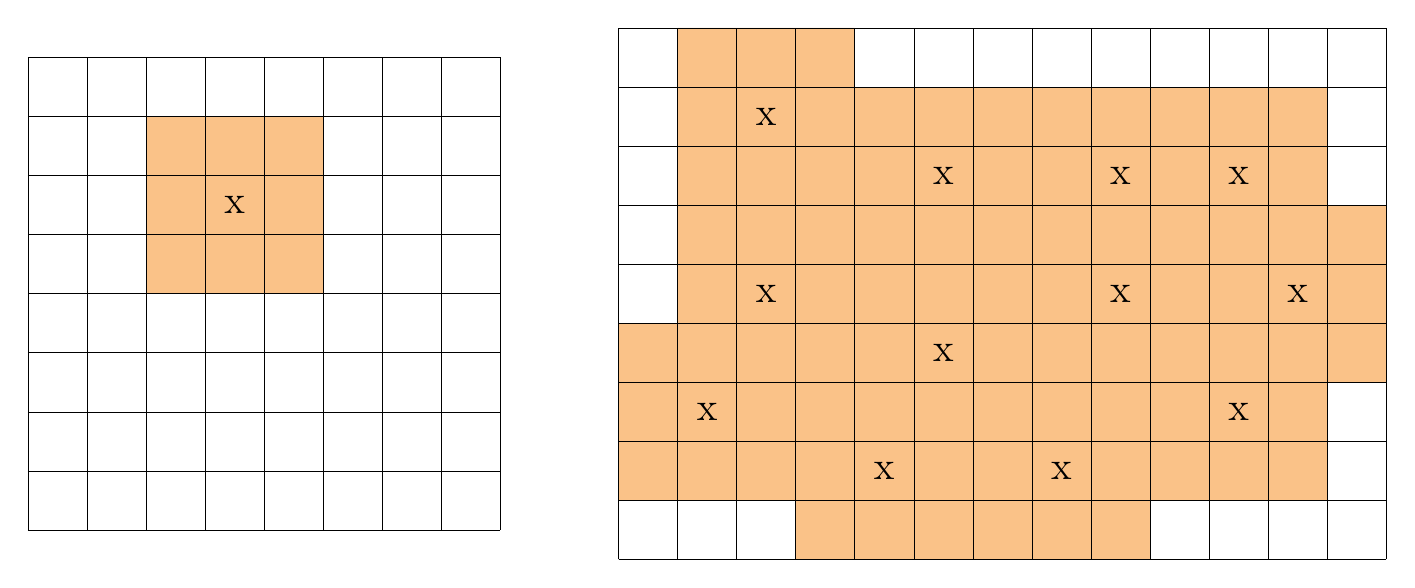
\begin{tikzpicture}[scale=0.75, main, line join=bevel]
		\begin{scope}
			\fill[BurntOrange, semitransparent] (2,4) rectangle (5,7);
			\draw[font=\small, main] (3.5,5.5) node {\Large x};
			\draw[main, very thin, xstep=1, ystep=1] (0,0) grid (8,8);
		\end{scope}
	
		\begin{scope}[xshift=10cm, yshift=-0.5cm]
			\fill[BurntOrange, semitransparent] (0,1) -- (3,1) -- (3,0) -- (9,0) -- (9,1) -- (12,1) -- (12,3) -- (13,3) -- (13,6) -- (12,6) -- (12,8) -- (4,8) -- (4,9) -- (1,9) -- (1,4) -- (0,4) -- cycle;
			\draw[font=\small, main] (4.5,1.5) node {\Large x};
			\draw[font=\small, main] (7.5,1.5) node {\Large x};
			\draw[font=\small, main] (10.5,2.5) node {\Large x};
			\draw[font=\small, main] (11.5,4.5) node {\Large x};
			\draw[font=\small, main] (10.5,6.5) node {\Large x};
			\draw[font=\small, main] (8.5,6.5) node {\Large x};
			\draw[font=\small, main] (5.5,6.5) node {\Large x};
			\draw[font=\small, main] (8.5,4.5) node {\Large x};
			\draw[font=\small, main] (5.5,3.5) node {\Large x};
			\draw[font=\small, main] (1.5,2.5) node {\Large x};
			\draw[font=\small, main] (2.5,4.5) node {\Large x};
			\draw[font=\small, main] (2.5,7.5) node {\Large x};
			\draw[main, very thin, xstep=1, ystep=1] (0,0) grid (13,9);
		\end{scope}
		
	\end{tikzpicture}
\end{document}